\section*{3. Random Variables}\label{random-variables}

\subsection*{3.1 Introduction}\label{introduction:RVs}
A \textbf{random variable} is a mapping \(X : \Omega \rightarrow \R\) that assigns a real number \(X(\omega)\) to each outcome \(\omega\).
\emph{Technically, a random variable must be measurable. See the technical appendix for details.}
Given a random variable \(X\) and a subset \(A\) of the real line, define \(X^{-1}(A) = \{ \omega \in \Omega : X(\omega) \in A \}\) and let
\begin{align*}
\PROB(X \in A) = \PROB(X^{-1}(A)) 
&= \PROB(\{ \omega \in \Omega; X(\omega) \in A \}) 
\\
\PROB(X = x) = \PROB(X^{-1}(x)) 
&= \PROB(\{ \omega \in \Omega; X(\omega) = x \})
\end{align*}
\(X\) denotes a random variable and \(x\) denotes a possible value of \(X\).

\subsection*{3.2 Distribution Functions and Probability Functions}\label{distribution:functions:probability}
The \textbf{cumulative distribution function}, CDF, \(F_X : \R \rightarrow [0, 1]\) of a random variable \(X\) is defined by
\[
F_X(x) = \PROB(X \leq x) 
\]
The following result shows that the CDF completely determines the distribution of a random variable.

\textbf{Theorem 3.7}. Let \(X\) have CDF \(F\) and let \(Y\) have CDF \(G\). If \(F(x) = G(x)\) for all \(x\) then \(\PROB(X \in A) = \PROB(Y \in A)\) for all \(A\).
\emph{Technically, we only have that \(\PROB(X \in A) = \PROB(Y \in A)\) for every measurable event \(A\).}

\textbf{Theorem 3.8}. A function \(F\) that maps the real line to \([0, 1]\) is a CDF for some probability measure \(\PROB\) if and only if if satisfies the following three conditions:
\begin{itemize}[tightlist]
\item
  \(F\) is non-decreasing, i.e.~\(x_{1} < x_{2}\) implies that
  \(F(x_{1}) \leq F(x_{2})\).
\item
  \(F\) is normalized: \(\lim_{n \rightarrow -\infty} F(x) = 0\) and
  \(\lim_{n \rightarrow +\infty} F(x) = 1\).
\item
  \(F\) is right-continuous, i.e.~\(F(x) = F(x^+)\) for all \(x\), where
\end{itemize}
\[
F(x^+) = \lim_{y \rightarrow x, y > x} F(y)
\]
\textbf{Proof}. Suppose that \(F\) is a CDF. Let us show that \(F\) is right-continuous. Let \(x\) be a real number and let \(y_{1}, y_{2}, \dots\) be a sequence of real numbers such that \(y_{1} > y_{2} > \dots\) and \(\lim_{i} y_{i} = x\). Let \(A_{i} = (-\infty, y_{i}]\) and let \(A = (-\infty, x]\). Note that \(A = \inter_{i=1}^{\infty} A_{i}\) and also note that \(A_{1} \supset A_{2} \supset \cdots\). Because the events are monotone, \(\lim_{i} \PROB(A_{i}) = \PROB(\inter_{i} A_{i})\). Thus,
\[
F(x) = \PROB(A) = \PROB(\inter_{i} A_{i}) = \lim_{i} \PROB(A_{i}) = \lim_{i} F(y_{i}) = F(x^+)
\]
Showing that \(F\) is non-decreasing and is normalized is similar. Proving the other direction, that is that \(F\) is non-decreasing, normalized, and right-continuous then it is a CDF for some random variable, uses some deep tools in analysis.
\(X\) is \textbf{discrete} if it takes countably many values
\[
\{ x_{1}, x_{2}, \dots \}
\]
We define the \textbf{probability density function} or
\textbf{probability mass function} for \(X\) by
\[
f_X(x) = \PROB(X = x)
\]
\emph{A set is countable if it is finite or if it can be put in a one-to-one correspondence with the integers.}
Thus, \(f_X(x) \geq 0\) for all \(x \in \R\) and \(\sum_{i} f_X(x_{i}) = 1\). The CDF of \(X\) is related to the PDF by
\[
F_X(x) = \PROB(X \leq x) = \sum_{x_{i} \leq x} f_X(x_{i})
\]
Sometimes we write \(f_X\) and \(F_X\) simply as \(f\) and \(F\).
A random variable \(X\) is \textbf{continuous} if there exists a function \(f_X\) such that \(f_X(x) \geq 0\) for all \(x\), \(\int_{-\infty}^{\infty} f_X(x) dx = 1\), and for every \(a \leq b\),
\[
\PROB(a < X < b) = \int_a^{b} f_X(x) dx
\]
The function \(f_X\) is called the \textbf{probability density function}. We have that
\[
F_X(x) = \int_{-\infty}^x f_X(t) dt
\]
and \(f_X(x) = F'_X(x)\) at all points \(x\) at which \(F_X\) is differentiable.
Sometimes we shall write \(\int f(x) dx\) or simply \(\int f\) to mean \(\int_{-\infty}^{\infty} f(x) dx\).
\textbf{Warning}: Note that if \(X\) is continuous then \(\PROB(X = x) = 0\) for every \(x\). We only have \(f(x) = \PROB(X = x)\) for discrete random variables; we get probabilities from a PDF by integrating.
\textbf{Lemma 3.15}. Let \(F\) be the CDF for a random variable \(X\).
Then:
\begin{itemize}
\item
  \(\PROB(X = x) = F(x) - F(x^-)\) where
  \(F(x^-) = \lim_{y \uparrow x} F(y)\)
\item
  \(\PROB(x < X \leq y) = F(y) - F(x)\)
\item
  \(\PROB(X > x) = 1 - F(x)\)
\item
  If \(X\) is continuous then
  \[
 \PROB(a < X < b) 
  = \PROB(a \leq X < b) 
  = \PROB(a < X \leq b) 
  = \PROB(a \leq X \leq b)
\]
\end{itemize}
It is also useful to define the inverse CDF (or quantile function).
Let \(X\) be a random variable with CDF \(F\). The \textbf{inverse CDF} or \textbf{quantile function} is defined by
\[
F^{-1}(q) = \inf \{ x : F(x) \ge q \}
\]
for \(q \in [0, 1]\). If \(F\) is strictly increasing and continuous then \(F^{-1}(q)\) is the unique real number \(x\) such that \(F(x) = q\).
We call \(F^{-1}(1/4)\) the first quartile, \(F^{-1}(1/2)\) the median (or second quartile), and \(F^{-1}(3/4)\) the third quartile.
Two random variables \(X\) and \(Y\) are \textbf{equal in distribution} -- denoted \(X \overset{d}= Y\) -- if \(F_X(x) = F_Y(x)\) for all \(x\). This does not mean that \(X\) and \(Y\) are equal. Rather, it means that probability statements about \(X\) and \(Y\) will be the same.

\subsection*{3.3 Some Important Discrete Random Variables}\label{some-important-discrete-random-variables}
\textbf{Notation}: It is traditional to write \(X \sim F\) to indicate that \(X\) has distribution \(F\). 
% This is an unfortunate notation since the symbol \(\sim\) is also used to denote an approximation. The notation is so pervasive we are stuck with it.
% Note: We use \(A \approx B\) to denote approximation. 
%The LaTeX macros hint at this common usage: \texttt{\textbackslash{}sim} for \(\sim\), and \texttt{\textbackslash{}approx} for \(\approx\).}
\paragraph{The Point Mass Distribution}\label{the-point-mass-distribution}
\(X\) has a point mass distribution at \(a\), denoted \(X \sim \delta_a\), if \(\PROB(X = a) = 1\), in which case
\[
F(x) = 
\begin{cases}
0 &\text{if } x < a 
\\[
1ex]
1 &\text{if } x \geq a
\end{cases}
\]
The probability mass function is \(f(x) = I(x = a)\), which takes value $1$ if \(x = a\) and 0 otherwise.
\paragraph{The Discrete Uniform Distribution}\label{the-discrete-uniform-distribution}
Let \(k > 1\) be a given integer. Suppose that \(X\) has probability mass function given by
\[
f(x) = 
\begin{cases}
1/k &\text{for } x = 1, \dots, k 
\\[
1ex]
0 &\text{otherwise}
\end{cases}
\]
We say that \(X\) has a uniform distribution on \(\{ 1, \dots, k \}\).
\paragraph{The Bernoulli Distribution}\label{the-bernoulli-distribution}
Let \(X\) represent a coin flip. Then \(\PROB(X = 1) = p\) and \(\PROB(X = 0) = 1 - p\) for some \(p \in [0, 1]\). We say that \(X\) has a Bernoulli distribution, denoted \(X \sim \text{Bernoulli}(p)\). The probability mass function is \(f(x) = p^x (1 - p)^{1 - x}\) for \(x \in \{ 0, 1 \}\).
\paragraph{The Binomial Distribution}\label{the-binomial-distribution}
Suppose we have a coin which falls heads with probability \(p\) for some \(0 \leq p \leq 1\). Flip the coin \(n\) times and let \(X\) be the number of heads. Assume that the tosses are independent. Let \(f(x) = \PROB(X = x)\) be the mass function. It can be shown that
\[
f(x) = 
\begin{cases}
\binomial{n}{x} p^x (1 - p)^{n - x} &\text{for } x= 0, \dots, n 
\\[
1ex]
0 &\text{otherwise}
\end{cases}
\]
A random variable with this mass function is called a Binomial random variable, and we write \(X \sim \text{Binomial}(n, p)\). If \(X_{1} \sim \text{Binomial}(n, p_{1})\) and \(X_{2} \sim \text{Binomial}(n, p_{2})\) then \(X_{1} + X_{2} \sim \text{Bimomial}(n, p_{1} + p_{2})\).
Note that \(X\) is a random variable, \(x\) denotes a particular value of the random variable, and \(n\) and \(p\) are \textbf{parameters}, that is, fixed real numbers.
\paragraph{The Geometric Distribution}\label{the-geometric-distribution}
\(X\) has a geometric distribution with parameter \(p \in (0, 1)\), denoted \(X \sim \text{Geom}(p)\), if
\[
\PROB(X = k) = p(1 - p)^{k - 1}, \quad k \geq 1
\]
We have that
\[
\sum_{k=1}^{\infty} \PROB(X = k) = p \sum_{k=1}^{\infty} (1 - p)^{k} = \frac{p}{1 - (1 - p)} = 1
\]
\(X\) counts the number of flips needed until the first head.
\paragraph{The Poisson Distribution}\label{the-poisson-distribution}
\(X\) has a Poisson distribution with parameter \(\lambda\), denoted \(X \sim \text{Poisson}(\lambda)\), if
\[
f(x) = e^{-\lambda} \frac{\lambda^x}{x!}, \quad x \geq 0
\]
Note that
\[
\sum_{x=1}^{\infty} f(x) 
= e^{-\lambda} \sum_{x=1}^{\infty} \frac{\lambda^x}{x!} 
= e^{-\lambda} e^\lambda = 1
\]
The Poisson distribution is often used as a model for counts of rare events like radioactive decay and traffic accidents. If \(X_{1} \sim \text{Poisson}(n, \lambda_{1})\) and \(X_{2} \sim \text{Poisson}(n, \lambda_{2})\) then \(X_{1} + X_{2} \sim \text{Poisson}(n, \lambda_{1} + \lambda_{2})\).
\textbf{Warning}: We defined random variables to be mappings from a sample space \(\Omega\) to \(\R\) but we did not mention sample space in any of the distributions above. Construct a sample space explicitly for a Bernoulli random variable. Let \(\Omega = [0, 1]\), and define \(\PROB\) to satisfy \(\PROB([a, b]) = b - a\) for \(0 \leq a \leq b \leq 1\). Fix \(p \in [0, 1]\) and define
\[
X(\omega) = 
\begin{cases}
1 &\text{if }\omega \leq p 
\\
0 &\text{if }\omega > p
\end{cases}
\]
Then \(\PROB(X = 1) = \PROB(\omega \leq p) = \PROB([0, p]) = p\) and \(\PROB(X = 0) = 1 - p\). Thus, \(X \sim \text{Bernoulli}(p)\). We could do this for all of the distributions defined above. In practice, we think of a random variable like a random number but formally it is a mapping defined on some sample space.

\subsection*{3.4 Some Important Continuous Random Variables}\label{some-important-continuous-random-variables}
\paragraph{The Uniform Distribution}\label{the-uniform-distribution}
\(X\) has a uniform distribution with parameters \(a\) and \(b\), denoted \(X \sim \text{Uniform}(a, b)\), if
\[
f(x) = 
\begin{cases}
\Frac{1}{b - a} &\text{for } x \in [a, b]
\\[
1ex]
0 &\text{otherwise}
\end{cases}
\]
where \(a < b\). The CDF is
\[
F(x) = 
\begin{cases}
0 &\text{if } x < a 
\\[
1ex]
\Frac{x - a}{b - a} &\text{if } x \in [a, b] 
\\[
1ex]
1 &\text{if } x > b
\end{cases}
\]
\paragraph{Normal (Gaussian)}\label{normal-gaussian}
\(X\) has a Normal (or Gaussian) distribution with parameters \(\mu\) and \(\sigma\), denoted by \(X \sim N(\mu, \sigma^{2})\), if
\[
f(x) = \frac{1}{\sigma \sqrt{2 \pi}} \exp \left\{ -\frac{1}{2} \left( \frac{x - \mu}{\sigma} \right)^{2}\right\}, \quad x \in \R
\]
where \(\mu \in \R\) and \(\sigma > 0\). Later we shall see that \(\mu\) is the ``center'' (or mean) of the distribution and that \(\sigma\) is the ``spread'' (or standard deviation) of the distribution. The Normal distribution plays an important role in probability and statistics. Many phenomena have approximately Normal distributions. Later, we shall see that the distribution of a sum of random variables can be approximated by a Normal distribution (the central limit Theorem).
We say that \(X\) has a \textbf{standard Normal distribution} if \(\mu = 0\) and \(\sigma = 1\). The standard Normal random variable is denoted by \(Z\). The PDF and the CDF of the standard Normal are denoted by \(\phi(z)\) and \(\Phi(z)\). The PDF is plotted below.

\begin{python}
import numpy as np
from scipy.stats import norm
import matplotlib.pyplot as plt
xx = np.arange(-5, 5, step=0.01)
plt.figure(figsize=(12, 8))
plt.plot(xx, norm.pdf(xx, loc=0, scale=1))
plt.title('Standard Normal PDF')
plt.show()
\end{python}

\begin{figure}[H]
\centering
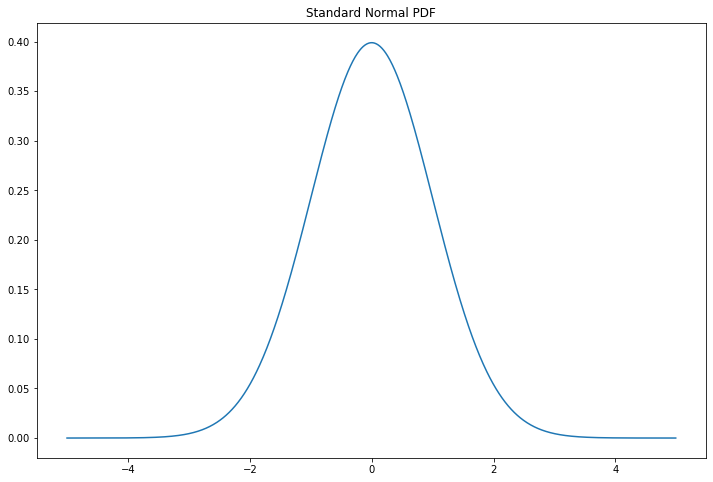
\includegraphics{Figure-03-01}
\end{figure}

There is no closed-form expression for \(\Phi\). Here are some useful facts:
\begin{itemize}
\item
  If \(X \sim N(\mu, \sigma^{2})\) then
  \(Z = (X - \mu) / \sigma \sim N(0, 1)\)
\item
  If \(Z \sim N(0, 1)\) then
  \(X = \mu + \sigma Z \sim N(\mu, \sigma^{2})\)
\item
  If \(X_{i} \sim N(\mu_{i}, \sigma_{i}^{2})\), \(i = 1, \dots, n\) are
  independent then
  \[
\sum_{i=1}^{n} X_{i} \sim N \left(\sum_{i=1}^{n} \mu_u, \sum_{i=1}^{n} \sigma_{i}^{2} \right)
\]
\end{itemize}
It follows from the first fact that if \(X \sim N(\mu, \sigma^{2})\) then
\[
\PROB(a < X < b) 
= \PROB\left( \frac{a - \mu}{\sigma} < Z < \frac{b - \mu}{\sigma} \right) 
= \Phi \left( \frac{b - \mu}{\sigma} \right) - \Phi \left( \frac{a - \mu}{\sigma} \right)
\]
Thus we can compute any probabilities we want as long as we can compute the CDF \(\Phi(z)\) of the standard Normal. All statistical and computing packages will compute \(\Phi(z)\) and \(\Phi^{-1}(q)\).
\paragraph{Exponential Distribution}\label{exponential-distribution}
\(X\) has an exponential distribution with parameter \(\beta\), denoted by \(X \sim \text{Exp}(\beta)\), if
\[
f(x) = \frac{1}{\beta} e^{-x / \beta}, \quad x > 0
\]
where \(\beta > 0\). The exponential distribution is used to model the lifetimes of electronic components and the waiting times between rare events.
\paragraph{Gamma Distribution}\label{gamma-distribution}
For \(\alpha > 0\), the \textbf{Gamma function} is defined by \(\Gamma(\alpha) = \int_{0}^{\infty} y^{\alpha - 1} e^{-y} dy\). \(X\) has a Gamma distribution with parameters \(\alpha\) and \(\beta\), denoted by \(X \sim \text{Gamma}(\alpha, \beta)\), if
\[
f(x) = \frac{1}{\beta^\alpha \Gamma(\alpha)} x^{\alpha - 1} e^{-x / \beta}, \quad x > 0
\]
where \(\alpha, \beta > 0\). The exponential distribution is just a \(\text{Gamma}(1, \beta)\) distribution. If \(X_{i} \sim \text{Gamma}(\alpha_{i}, \beta)\) are independent, then \(\sum_{i=1}^{n} X_{i} \sim \text{Gamma}\left( \sum_{i=1}^{n} \alpha_{i}, \beta \right)\).
\paragraph{Beta Distribution}\label{beta-distribution}
\(X\) has Beta distribution with parameters \(\alpha > 0\) and \(\beta > 0\), denoted by \(X \sim \text{Beta}(\alpha, \beta)\), if
\[
f(x) = \frac{\Gamma(\alpha + \beta)}{\Gamma(\alpha) \Gamma(\beta)} x^{\alpha - 1} (1 - x)^{\beta - 1}, \quad 0 < x < 1
\]
\paragraph{\texorpdfstring{\(t\) and Cauchy Distribution}{t and Cauchy Distribution}}\label{t-and-cauchy-distribution}
\(X\) has a \(t\) distribution with \(\nu\) degrees of freedom -- denoted \(X \sim t_\nu\), if
\[
f(x) = \frac{1}{\sqrt{\nu \pi}} \frac{\Gamma\left( \frac{\nu + 1}{2} \right)}{\Gamma\left( \frac{\nu}{2} \right)} \frac{1}{\left(1 + \frac{x^{2}}{\nu} \right)^{(\nu + 1) / 2}} 
\]
The \(t\) distribution is similar to a Normal but it has thicker tails. In fact, the Normal corresponds to a \(t\) with \(\nu = \infty\). The Cauchy distribution is a special case of the \(t\) distribution corresponding to \(\nu = 1\). The density is
\[
f(x) = \frac{1}{\pi (1 + x^{2})}
\]
\paragraph{\texorpdfstring{The \(\chi^{2}\) Distribution}{The \textbackslash chi^{2} Distribution}}\label{chi2:dist}
\(X\) has a \(\chi^{2}\) distribution with \(p\) degrees of freedom -- denoted \(X \sim \chi_{p}^{2}\) -- if
\[
f(x) = \frac{1}{\Gamma\left(\frac{p}{2}\right) 2^{\frac{p}{2}}} x^{\frac{p}{2} - 1} e^{-\frac{x}{2}}, \quad x > 0 
\]
If \(Z_{1}, Z_{2}, \dots\) are independent standard Normal random variables then \(\sum_{i=1}^p Z_{i}^{2} \sim \chi_{p}^{2}\).

\subsection*{3.5 Bivariate Distributions}\label{bivariate-distributions}
Given a pair of discrete random variables \(X\) and \(Y\), define the \textbf{joint mass function} by \(f(x, y) = \PROB(X = x \text{ and } Y = y)\). From now on, we write \(\PROB(X = x \text{ and } Y = y)\) as \(\PROB(X = x, Y = y)\). We write \(f\) as \(f_{X, Y}\) when we want to be more explicit.
In the continuous case, we call a function \(f(x, y)\) a PDF for the random variables \((X, Y)\) if:  \(f(x, y) \geq 0\) for all \((x, y)\), \( \int_{-\infty}^{\infty}\int_{-\infty}^{\infty} f(x, y) dx dy = 1\) 
For any set \(A \subset \R \times \R\), \(\PROB((X, Y) \in A) = \int \int_A f(x, y) \; dx dy\)
In the continuous or discrete case, we define the joint CDF as 
\(F_{X, Y}(x, y) = \PROB(X \leq x, Y \leq y)\).

\subsection*{3.6 Marginal Distributions}\label{marginal-distributions}
If \((X, Y)\) have joint distribution with mass function \(f_{X, Y}\), then the \textbf{marginal mass function} for \(X\) is defined by
\[
f_X(x) = \PROB(X = x) = \sum_y \PROB(X = x, Y = y) = \sum_y f(x, y)
\]
and the \textbf{marginal mass function} for \(Y\) is defined by
\[
f_Y(y) = \PROB(Y = y) = \sum_x \PROB(X = x, Y = y) = \sum_x f(x, y) 
\]
For continuous random variables, the marginal densities are
\[
f_X(x) = \int f(x, y) \; dy \quad \text{and} \quad f_Y(y) = \int f(x, y) \; dx 
\]
The corresponding marginal CDFs are denoted by \(F_X\) and \(F_Y\).

\subsection*{3.7 Independent Random Variables}\label{independent-random-variables}
Two random variables \(X\) and \(Y\) are \textbf{independent} if, for every \(A\) and \(B\),
\[
\PROB(X \in A, Y \in B) = \PROB(X \in A) \PROB(Y \in B)
\]
We write \(X \ci Y\).
In principle, to check whether \(X\) and \(Y\) are independent we need to check the equation above for all subsets \(A\) and \(B\). Fortunately, we have the following result which we state for continuous random variables though it is true for discrete random variables too.

\textbf{Theorem 3.30}. Let \(X\) and \(Y\) have joint PDF \(f_{X, Y}\). Then \(X \ci Y\) if and only if \(f_{X, Y}(x, y) = f_X(x) f_Y(y)\) for all values \(x\) and \(y\).
\emph{The statement is not rigorous because the density is defined only up to sets of measure 0.}
The following result is helpful for verifying independence.

\textbf{Theorem 3.33}. Suppose that the range of \(X\) and \(Y\) is a (possibly infinite) rectangle. If \(f(x, y) = g(x) h(y)\) for some functions \(g\) and \(h\) (not necessarily probability density functions) then \(X\) and \(Y\) are independent.

\subsection*{3.8 Conditional Distributions}\label{conditional-distributions}
The \textbf{conditional probability mass function} is
\[
f_{X | Y}(x | y) = \PROB(X = x | Y = y) = \frac{\PROB(X = x, Y = y)}{\PROB(Y = y)} = \frac{f_{X, Y}(x, y)}{f_Y(y)}
\]
if \(f_Y(y) > 0\).
For continuous random variables, the \textbf{conditional probability density function} is
\[
f_{X | Y}(x | y) = \frac{f_{X, Y}(x, y)}{f_Y(y)}
\]
assuming that \(f_Y(y) > 0\). Then,
\[
\PROB(X \in A | Y = y) = \int_A f_{X | Y}(x | y) \; dx
\]
\emph{We are treading in deep water here. When we compute \(\PROB(X \in A | Y = y)\) in the continuous case we are conditioning on the event \(\PROB(Y = y)\) which has probability $0$. We avoid this problem by defining things in terms of the PDF. The fact that this leads to a well-defined theory is proved in more advanced courses. We simply take it as a definition.}

\subsection*{3.9 Multivariate Distributions and IID Samples}\label{multivariate-distributions-and-iid-samples}
Let \(X = (X_{1}, \dots, X_{n})\) where the \(X_{i}\)s are random variables. We call \(X\) a \textbf{random vector}. Let \(f(x_{1}, \dots, x_{n})\) denote the PDF. It is possible to define their marginals, conditionals, etc. much the same way as in the bivariate case. We say that \(X_{1}, \dots, X_{n}\) are independent if, for every \(A_{1}, \dots, A_{n}\),
\[
\PROB(X_{1} \in A_{1}, \dots, X_{n} \in A_{n}) = \prod_{i=1}^{n} \PROB(X_{i} \in A_{i})
\]
It suffices to check that \(f(x_{1}, \dots, x_{n}) = \prod_{i=1}^{n} f_{X_{i}}(x_{i})\). If \(X_{1}, \dots, X_{n}\) are independent and each has the same marginal distribution with density \(f\), we say that \(X_{1}, \dots, X_{n}\) are IID (independent and identically distributed). We shall write this as \(X_{1}, \dots, X_{n} \sim f\) or, in terms of the CDF, \(X_{1}, \dots, X_{n} \sim F\). This means that \(X_{1}, \dots, X_{n}\) are independent draws from the same distribution. We also call \(X_{1}, \dots, X_{n}\) a \textbf{random sample} from \(F\).

\subsection*{3.10 Two Important Multivariate Distributions}\label{two-important-multivariate-distributions}
\paragraph{Multinomial Distribution}\label{multinomial-distribution}
The multivariate version of the Binomial is called a Multinomial.
Consider drawing a ball from an urn which has balls of \(k\) different
colors. Let \(p = (p_{1}, \dots, p_{k})\) where \(p_{j} \geq 0\) and
\(\sum_{j=1}^{k} p_{j} = 1\) and suppose that \(p_{j}\) is the probability of
drawing a ball of color \(j\). Draw \(n\) times (independent draws with
replacement) and let \(X = (X_{1}, \dots, X_{k})\), where \(X_{j}\) is the
number of times that color \(j\) appears. Hence,
\(n = \sum_{j=1}^{k} X_{j}\). We say that \(X\) has a Multinomial
distribution with parameters \(n\) and \(p\), denoted
\(X \sim \text{Multinomial}(n, p)\). The probability function is
\[
f(x) = \binom{n}{x_{1} \cdots x_{k}} p_{1}^{x_{1}} \cdots p_{k}^{x_{k}}
\]
where
\[
\binom{n}{x_{1} \cdots x_{k}} = \frac{n!}{x_{1}! \cdots x_{k}!}
\]
\textbf{Lemma 3.41}. Suppose that \(X \sim \text{Multinomial}(n, p)\)
where \(X = (X_{1}, \dots, X_{k})\) and \(p = (p_{1}, \dots, p_{k})\). The
marginal distribution of \(X_{j}\) is \(\text{Binomial}(n, p_{j})\).
\paragraph{Multivariate Normal}\label{rv:multivariate:normal}
The univariate Normal had two parameters, \(\mu\) and \(\sigma\). In the
multivariate vector, \(\mu\) is a vector and \(\sigma\) is replaced by a
matrix \(\Sigma\). To begin, let
\[
Z = \begin{pmatrix}
Z_{1} \\
\vdots \\
Z_{k}
\end{pmatrix}
\]
where \(Z_{1}, \dots, Z_{k} \sim N(0, 1)\) are independent. The density of
\(Z\) is
\[
f(z) = \prod_{i=1}^{k} f(z_{i}) 
= \frac{1}{(2 \pi)^{k/2}} \exp \left\{ -\frac{1}{2} \sum_{j=1}^{k} z_{j}^{2} \right\} 
= \frac{1}{(2 \pi)^{k/2}} \exp \left\{ -\frac{1}{2} z^T z \right\} 
\]
We say that \(Z\) has a standard multivariate Normal distribution, denoted \(Z \sim N(0, I)\) where it is understood that \(0\) represents a vector of \(k\) zeroes and \(I\) is the \(k \times k\) identity matrix.
More generally, a vector \(X\) has multivariate Normal distribution, denoted by \(X \sim N(\mu, \Sigma)\), if it has density
\[
f(x; \mu, \Sigma) = \frac{1}{(2 \pi)^{k/2} \det(\Sigma)^{1/2}} \exp \left\{ - \frac{1}{2} (x - \mu)^T \Sigma^{-1} (x - \mu) \right\}
\]
where \(\det(\cdot)\) denotes the determinant of a matrix, \(\mu\) is a vector of length \(k\), and \(\Sigma\) is a \(k \times k\) symmetric, positive definite matrix. Setting \(\mu = 0\) and \(\Sigma = I\) gives back the standard Normal.
\emph{A matrix \(\Sigma\) is positive definite if, for all non-zero vectors \(x\), \(x^T \Sigma x > 0\).}
Since \(\Sigma\) is symmetric and positive definite, it can be shown that there exists a matrix \(\Sigma^{1/2}\) -- called the square root of \(\Sigma\) -- with the following properties:
\begin{itemize}[tightlist]
\item
  \(\Sigma^{1/2}\) is symmetric
\item
  \(\Sigma = \Sigma^{1/2} \Sigma^{1/2}\)
\item
  \(\Sigma^{1/2}\Sigma^{-1/2} = \Sigma^{-1/2}\Sigma^{1/2} = I\), where
  \(\Sigma^{1/2} = \left(\Sigma^{1/2}\right)^{-1}\)
\end{itemize}

\textbf{Theorem 3.42}. If \(Z \sim N(0, I)\) and
\(X = \mu + \Sigma^{1/2} Z\) then \(X \sim N(\mu, \Sigma)\). Conversely,
if \(X \sim N(\mu, \Sigma)\), then
\(\Sigma^{-1/2}(X - \mu) \sim N(0, I)\).
Suppose we partition a random Normal vector \(X\) as \(X = (X_a, X_b)\),
and we similarly partition
\[
\mu = \begin{pmatrix}\mu_a & \mu_b \end{pmatrix} 
\quad
\Sigma = \begin{pmatrix}
\Sigma_{aa} & \Sigma_{ab} \\
\Sigma_{ba} & \Sigma_{bb}
\end{pmatrix}
\]

\textbf{Theorem 3.43}. Let \(X \sim N(\mu, \Sigma)\). Then:
\begin{enumerate}[label={\arabic*.}]
\item
  The marginal distribution of \(X_a\) is
  \(X_a \sim N(\mu_a, \Sigma_{aa})\).
\item
  The conditional distribution of \(X_b\) given \(X_a = x_a\) is
  \[
 X_b | X_a = x_a \sim N \left( \mu_b + \Sigma_{ba}\Sigma_{aa}^{-1}(x_a - \mu_a), \Sigma_{bb} - \Sigma_{ba} \Sigma_{aa}^{-1} \Sigma_{ab} \right)
\]
\item
  If \(a\) is a vector then \(a^T X \sim N(a^T \mu, a^T \Sigma a)\)
\item
  \(V = (X - \mu)^T \Sigma^{-1} (X - \mu) \sim \chi_{k}^{2}\)
\end{enumerate}

\subsection*{3.11 Transformations of Random
Variables}\label{transformations-of-random-variables}
Suppose that \(X\) is a random variable with PDF \(f_X\) and CDF
\(F_X\). Let \(Y = r(X)\) be a function of \(X\), such as \(Y = X^{2}\) or
\(Y = e^X\). We call \(Y = r(X)\) a transformation of \(X\). How do we
compute the PDF and the CDF of \(Y\)? In the discrete case, the answer
is easy. The mass function of \(Y\) is given by
\[
f_Y(y) = \PROB(Y = y) = \PROB(r(X) = y) = \PROB(\{x; r(x) = y\}) = \PROB(X \in r^{-1}(y))
\]
The continuous case is harder. There are 3 steps for finding \(f_Y\):
\begin{enumerate}[label={\arabic*.}]
\item
  For each \(y\), find the set \(A_y = \{ x : r(x) \leq y \}\).
\item
  Find the CDF
  \[
F_Y(y) = \PROB(Y \leq y) = \PROB(r(X) \leq y) = \PROB(\{x ; r(x) \leq y \}) = \int_{A_y} f_X(x) dx
\]
\item
  The PDF is \(f_Y(y) = F'_Y(y)\).
\end{enumerate}
When \(r\) is strictly monotone increasing or strictly monotone
decreasing then \(r\) has an inverse \(s = r^{-1}\) and in this case one
can show that
\[
f_Y(y) = f_X(s(y)) \;\Bigg| \frac{ds(y)}{dy} \Bigg|
\]

\subsection*{3.12 Transformation of Several Random
Variables}\label{transformation-of-several-random-variables}
In some cases we are interested in the transformation of several random
variables. For example, if \(X\) and \(Y\) are given random variables,
we might want to know the distribution of \(X / Y\), \(X + Y\),
\(\max \{ X, Y \}\) or \(\min \{ X, Y \}\). Let \(Z = r(X, Y)\). The
steps for finding \(f_Z\) are the same as before:
\begin{enumerate}[tightlist,label={\arabic*.}]
\item
  For each \(z\), find the set \(A_z = \{ (x, y) : r(x, y) \leq z \}\).
\item
  Find the CDF
\end{enumerate}
\[
F_Z(z) = \PROB(Z \leq z) = \PROB(r(X, Y) \leq z) = \PROB(\{ (x, y) : r(x, y) \leq z \})
  = \int \int_{A_z} f_{X, Y}(x, y) \; dx dy 
\]
\begin{enumerate}[tightlist,label={\arabic*.},resume]
\item
  Find \(f_Z(z) = F'_Z(z)\).
\end{enumerate}

\subsection*{3.13 Technical Appendix}
Recall that a probability measure \(\PROB\) is defined on a
\(\sigma\)-field \(\mathcal{A}\) of a sample space \(\Omega\). A random
variable \(X\) is \textbf{measurable} map
\(X : \Omega \rightarrow \R\). Measurable means that, for every
\(x\), $\{ \omega : X(\omega) \leq x \} \in \mathcal{A} $.

\subsection*{3.14 Exercises}

\textbf{Exercise 3.14.1}. Show that
\[
\PROB(X = x) = F(x^+) - F(x^-)
\]
and
\[
F(x_{2}) - F(x_{1}) = \PROB(X \leq x_{2}) - \PROB(X \leq x_{1})
\]

\textbf{Solution}.
By definition, \(F(x_{2}) = \PROB(X \leq x_{2})\) and
\(F(x_{1}) = \PROB(X \leq x_{1})\), so the second equation is
immediate.
Also by definition,
\[
F(x^+) = \lim_{y \rightarrow x, y > x} F(y) = \lim_{y \rightarrow x, y > x} \PROB(X \leq y) 
= \PROB(\exists y : X \leq y, y > x) 
= \PROB(X \leq x)
\]
and
\[
F(x^-) = \lim_{y \rightarrow x, y < x} F(y) = \lim_{y \rightarrow x, y > x} \PROB(X \leq y) 
= \PROB(\exists y : X \leq y, y < x)
= \PROB(X < x)
\]
and so
\[
F(x^+) - F(x^-) = \PROB(X \leq x) - \PROB(X < x) = \PROB(X(\omega) \in \{x : X(\omega) \leq x \} - \{x: X(\omega) < x \}) = \PROB(X = x)
\]

\textbf{Exercise 3.14.2}. Let \(X\) be such that
\(\PROB(X = 2) = \PROB(X = 3) = 1/10\) and
\(\PROB(X = 5) = 8/10\). Plot the CDF \(F\). Use \(F\) to find
\(\PROB(2 < X \leq 4.8)\) and \(\PROB(2 \leq X \leq 4.8)\).

\textbf{Solution}.

\begin{python}
import numpy as np
import matplotlib.pyplot as plt
plt.figure(figsize=(12, 8))
# Draw horizontal lines
for xmin, xmax, y in [(0, 2, 0), (2, 3, 1/10), (3, 5, 2/10), (5, 10, 1)]:
    plt.hlines(y, xmin, xmax, color='C0', linestyle='solid')
    
# Draw vertical lines
for ymin, ymax, x in [(0, 1/10, 2), (1/10, 2/10, 3), (2/10, 1, 5)]:
    plt.vlines(x, ymin, ymax, color='C0', linestyle='dashed')
    
# Mark open intervals
plt.scatter([2, 3, 5], [0, 1/10, 2/10], color='C0', facecolor='white', zorder=10, linewidth=2)
# Mark close intervals
plt.scatter([2, 3, 5], [1/10, 2/10, 1], color='C0', facecolor='C0', zorder=10, linewidth=2)
plt.xlabel('x')
plt.ylabel('F(x)')
plt.show()
\end{python}

\begin{figure}[H]
\centering
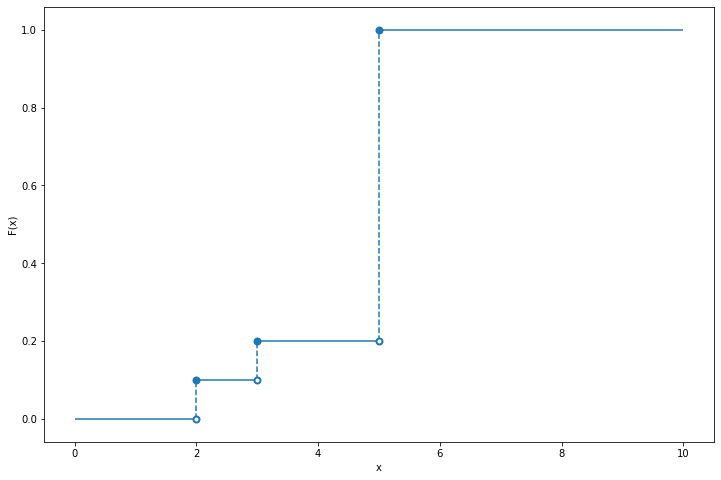
\includegraphics{Figure-03-02}
\end{figure}

\begin{align*}
\PROB(2 < X \leq 4.8) 
& = F(4.8) - F(2) = 0.2 - 0.1 = 0.1
\\
\PROB(2 \leq X \leq 4.8) 
& = F(4.8) - F(2^{-}) = 0.2 - 0 = 0.2
\end{align*}

\textbf{Exercise 3.14.3}. Prove Lemma 3.15.
Let \(F\) be the CDF for a random variable \(X\). Then:
\begin{itemize}
\item
  \(\PROB(X = x) = F(x) - F(x^-)\) where
  \(F(x^-) = \lim_{y \uparrow x} F(y)\)
\item
  \(\PROB(x < X \leq y) = F(y) - F(x)\)
\item
  \(\PROB(X > x) = 1 - F(x)\)
\item
  If \(X\) is continuous then
  \[
\PROB(a < X < b) = \PROB(a \leq X < b) = \PROB(a < X \leq b) = \PROB(a \leq X \leq b)
\]
\end{itemize}

\textbf{Solution}.
Proof of first statement:
\[
F(x) - F(x^{-}) = \PROB(X \leq x) - \PROB(X < x) = \PROB(\{\omega : X(\omega) \leq x\} - \{\omega : X(\omega) < x\}) = \PROB(X = x)
\]
Proof of second statement:
\[
\PROB(x < X \leq y) = \PROB(\{\omega : X(\omega) \leq y\} - \{\omega : X(\omega) \leq x\}) = \PROB(X \leq y) - \PROB(X \leq x) = F(y) - F(x)
\]
Proof of third statement:
\[
\PROB(X > x) = \PROB(\{\omega: X(\omega) > x\}) = \PROB(\{\omega: X(\omega) \leq x\}^{c}) = 1 - \PROB(X \leq x) = 1 - F(x)
\]
Proof of fourth statement:
If \(F\) is continuous, then
\(\PROB(X = a) = \PROB(X = b) = 0\), and so
\begin{align*}
\PROB(a < X \leq b) 
&= \PROB(a < X < b) + \PROB(X = b) = \PROB(a < X < b) 
\\
\PROB(a \leq X < b) 
&= \PROB(X = a) + \PROB(a < X < b) = \PROB(a < X < b) 
\\
\PROB(a \leq X \leq b) 
&= \PROB(X = a) + \PROB(a < X < b) + \PROB(X = b) 
 = \PROB(a < X < b)
\end{align*}

\textbf{Exercise 3.14.4}. Let \(X\) have probability density function
\[
f_X(x) = 
\begin{cases}
1/4 &\text{if } 0 < x < 1 \\
3/8 &\text{if } 3 < x < 5 \\
0   &\text{otherwise}
\end{cases}
\]
\textbf{(a)} Find the cumulative distribution function of \(X\).
\textbf{(b)} Let \(Y = 1 / X\). Find the probability density function
\(f_Y(y)\) for \(Y\). Hint: Consider three cases,
\(\frac{1}{5} \leq y \leq \frac{1}{3}\), \(\frac{1}{3} \leq y \leq 1\),
and \(y \geq 1\).

\textbf{Solution}.
\textbf{(a)}
\[
F_X(x) = 
\begin{cases}
0 &\text{if } x \leq 0 \\
\Frac{x}{4} &\text{if } 0 < x \leq 1 \\
\Frac{1}{4} &\text{if } 1 < x \leq 3 \\
\Frac{1}{4} + \frac{3(x - 3)}{8} &\text{if } 3 < x \leq 5 \\
1 &\text{if } x \geq 5
\end{cases} 
\]

\begin{python}
import numpy as np
import matplotlib.pyplot as plt
plt.figure(figsize=(12, 8))
# Draw horizontal lines
for xmin, xmax, y in [(-2, 0, 0), (1, 3, 1/4), (5, 7, 1)]:
    plt.hlines(y, xmin, xmax, color='C0', linestyle='solid')
    
# Draw diagonal lines
for x1, y1, x2, y2 in [(0, 0, 1, 1/4), (3, 1/4, 5, 1)]:
    plt.plot([x1, x2], [y1, y2], color='C0')
    
plt.xlabel(r'$x$')
plt.ylabel(r'$F(x)$')
plt.show()
\end{python}

\begin{figure}[H]
\centering
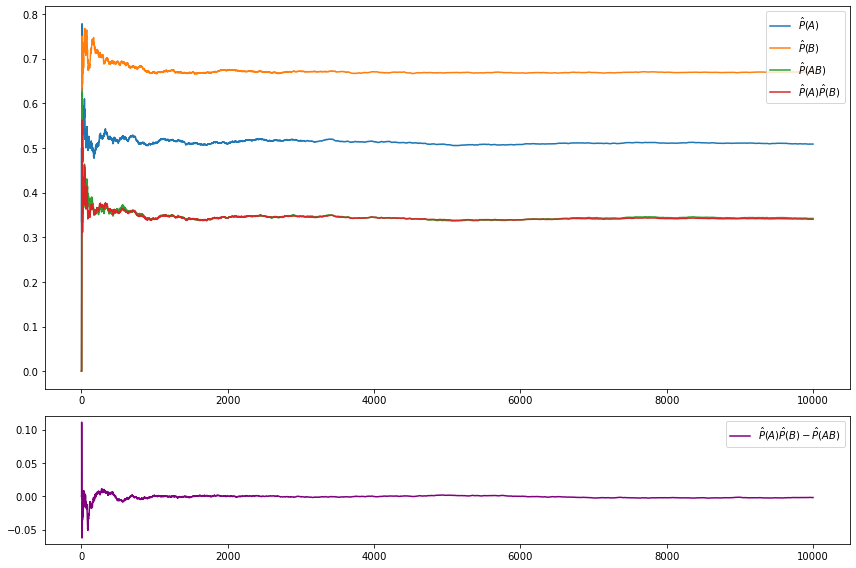
\includegraphics{Figure-02-03}
\end{figure}

\textbf{(b)}
\(\PROB(X > 0) = 1\), so \(\PROB(Y > 0) = 1\). For \(y > 0\),
we have:
\[
F_Y(y) = \PROB(Y \leq y) 
= \PROB\left(\frac{1}{X} \leq y\right) 
= \PROB\left(X \geq \frac{1}{y}\right) 
= 1 - F_X\left(\frac{1}{y} \right)
\]
so
\[
F_Y(y) = 
\begin{cases}
0 
&\text{if } y \leq \Frac{1}{5} \\
\Frac{15}{8} - \frac{3}{8y} 
&\text{if } \frac{1}{5} < y \leq \frac{1}{3} \\
\Frac{3}{4} 
&\text{if } \frac{1}{3} < y \leq 1 \\
1 - \Frac{1}{4y} 
&\text{if } y > 1
\end{cases}
\]

\begin{python}
import numpy as np
import matplotlib.pyplot as plt
plt.figure(figsize=(12, 8))
# Draw horizontal lines
for xmin, xmax, y in [(-2, 1/5, 0), (1/3, 1, 3/4)]:
    plt.hlines(y, xmin, xmax, color='C0')
    
# Draw increasing segments
yy = np.arange(1/5, 1/3, step=0.001)
plt.plot(yy, 15/8 - 3/(8 * yy), color='C0')
yy = np.arange(1, 8, step=0.01)
plt.plot(yy, 1 - 1/(4*yy), color='C0')
    
plt.xlabel(r'$y$')
plt.ylabel(r'$F_Y(y)$')
plt.show()
\end{python}

\begin{figure}[H]
\centering
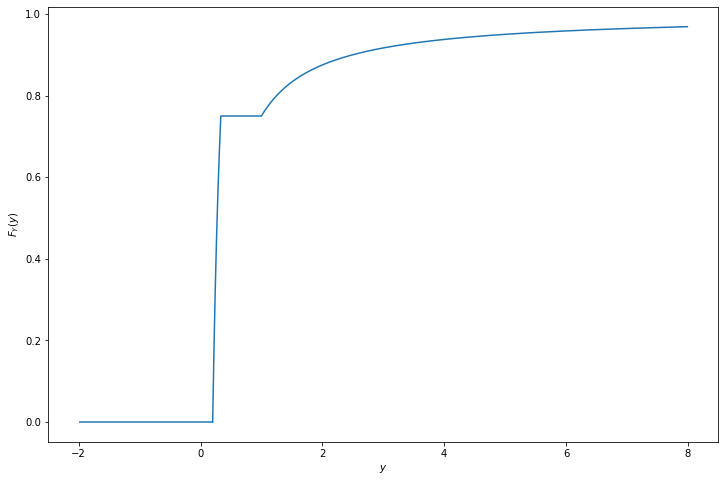
\includegraphics{Figure-03-04}
\end{figure}

The probability density function is \(f_y(y) = F'_Y(y)\), so
\[
f_Y(y) = 
\begin{cases}
0
&\text{if } y \leq \frac{1}{5} \\
\frac{3}{8y^{2}} 
&\text{if } \frac{1}{5} < y \leq \frac{1}{3} \\
0 
&\text{if } \frac{1}{3} < y \leq 1 \\
\frac{1}{4y^{2}} 
&\text{if } y > 1
\end{cases}
\]

\begin{python}
import numpy as np
import matplotlib.pyplot as plt
def f_Y(y):
    return np.where(y <= 1/5, 0, np.where(y <= 1/3, 3/(8 * (y**2)), 
                    np.where(y <= 1, 0, 1/(4 * (y**2)))))
plt.figure(figsize=(12, 8))
yy = np.arange(-1, 3, step=0.001)
plt.plot(yy, f_Y(yy), color='C0')
    
plt.xlabel(r'$y$')
plt.ylabel(r'$f_Y(y)$')
plt.show()
\end{python}

\begin{figure}[H]
\centering
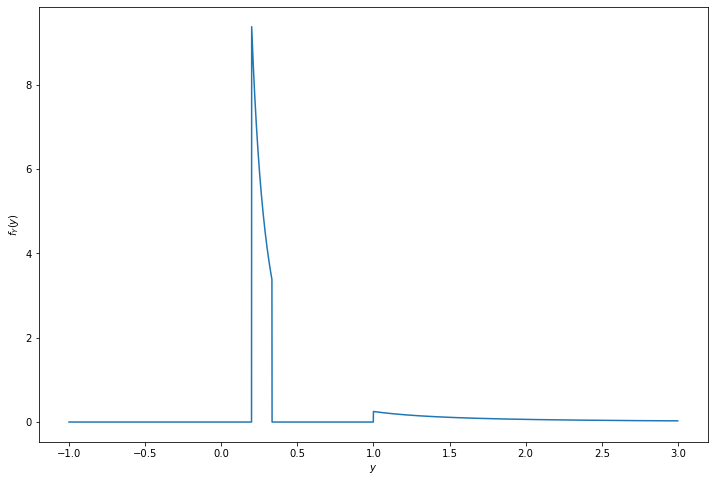
\includegraphics{Figure-03-05}
\end{figure}


\textbf{Exercise 3.14.5}. Let \(X\) and \(Y\) be discrete random
variables. Show that \(X\) and \(Y\) are independent if and only if
\(f_{X, Y}(x, y) = f_X(x) f_Y(y)\) for all \(x\) and \(y\).

\textbf{Solution}. If \(x\) or \(y\) take values that have probability
mass 0, then trivially \(f_{X, Y}(x, y) = 0\) and \(f_X(x) f_Y(y) = 0\),
so we only need to consider \(x\) and \(y\) with positive probability
mass.
If \(X\) and \(Y\) are independent, then
\(\PROB(X \in A, Y \in B) = \PROB(X \in A)\PROB(Y \in B)\)
for all events \(A\), \(B\). In particular, this is true for
\(A = \{x\}\) and \(B = \{ y \}\) for all \(x, y\), proving the
implication in one direction.
In the other direction, we have
\[
\PROB(X \in A, Y \in B) = \sum_{x \in A} \sum_{y \in B} f_{X, Y}(x, y)
\]
and
\[
\PROB(X \in A) = \sum_{x \in A} f_X(x)
\quad \text{and} \quad
\PROB(Y \in B) = \sum_{y \in B} f_Y(y)
\]
so \(f_{X, Y}(x, y) = f_X(x) f_Y(y)\) for all \(x, y\) implies that for
all \(A\) and \(B\),
\begin{align*}
\PROB(X \in A) \PROB(Y \in B) 
& = \left( \sum_{x \in A} f_X(x) \right) \left( \sum_{y \in B} f_Y(y) \right)
\\
& = \sum_{x \in A} \sum_{y \in B} f_X(x) f_Y(y) 
\\
& = \sum_{x \in A} \sum_{y \in B} f_{X, Y}(x, y) = \PROB(X \in A, Y \in B)
\end{align*}
so \(X, Y\) are independent, proving the implication in the other
direction.

\textbf{Exercise 3.14.6}. Let \(X\) have distribution \(F\) and density
function \(f\) and let \(A\) be a subset of the real line. Let
\(I_A(x)\) be the indicator function for \(A\):
\[
I_A(x) = \begin{cases}
1 &\text{if } x \in A 
\\[
1ex]
0 &\text{otherwise}
\end{cases}
\]
Let \(Y = I_A(X)\). Find an expression for the cumulative distribution
function of \(Y\). (Hint: first find the mass function for \(Y\).)

\textbf{Solution}. Note that \(I_A\) can only return values 0 or 1, so
\(Y\) is a discrete variable with non-zero probability mass only at
values 0 and 1.
But $\PROB(Y = 1) = \PROB(x \in A) = \int\_A f\_X(x) dx $,
so the PDF for \(Y\) is:
\[
f_Y(y) = \begin{cases}
\int_A f_X(x) dx &\text{if } y = 1 \\
1 - \int_A f_X(x) dx &\text{if } y = 0 \\
0 &\text{otherwise}
\end{cases}
\]
and so the CDF of \(Y\) is:
\[
F_Y(y) = \begin{cases}
0 &\text{if } y < 0 \\
1 - \int_A f_X(x) dx &\text{if } 0 \leq y < 1 \\
1 &\text{if } y \geq 1
\end{cases}
\]

\textbf{Exercise 3.14.7}. Let \(X\) and \(Y\) be independent and suppose
that each has a \(\text{Uniform}(0, 1)\) distribution. Let
\(Z = \min \{ X, Y \}\). Find the density \(f_Z(z)\) for \(Z\). Hint: it
might be easier to first find \(\PROB(Z > z)\).

\textbf{Solution}.
\[
1 - F_Z(z) = \PROB(Z > z) = \PROB(X > z, Y > z) = (1 - F_X(z)) (1 - F_Y(z))
\]
But \(F_X\) and \(F_Y\) are both the CDF of the \(\text{Uniform}(0, 1)\)
distribution, so
\[
F_X(x) = \begin{cases}
0 &\text{if } x \leq 0 \\
x &\text{if } 0 < x \leq 1 \\
1 &\text{if } x > 1
\end{cases}
\]
and so
\[
F_Z(z) = \begin{cases}
0 &\text{if } z \leq 0 \\
2z - z^{2} &\text{if } 0 < z \leq 1 \\
1 &\text{if } z > 1
\end{cases}
\]
and the PDF is \(f_Z(z) = F'_Z(z)\):
\[
f_Z(z) = \begin{cases}
0 &\text{if } z \leq 0 \\
2 - 2z &\text{if } 0 < z < 1 \\
0 &\text{if } z > 1
\end{cases}
\]

\begin{python}
import numpy as np
import matplotlib.pyplot as plt
def f_Z(z):
    return np.where(z <= 0, 0, np.where(z >= 1, 0, 2 - 2 * z))
plt.figure(figsize=(12, 8))
zz = np.arange(-0.5, 1.5, step=0.01)
plt.plot(zz, f_Z(zz), color='C0')
    
plt.xlabel(r'$z$')
plt.ylabel(r'$f_Z(z)$')
plt.show()
\end{python}

\begin{figure}[H]
\centering
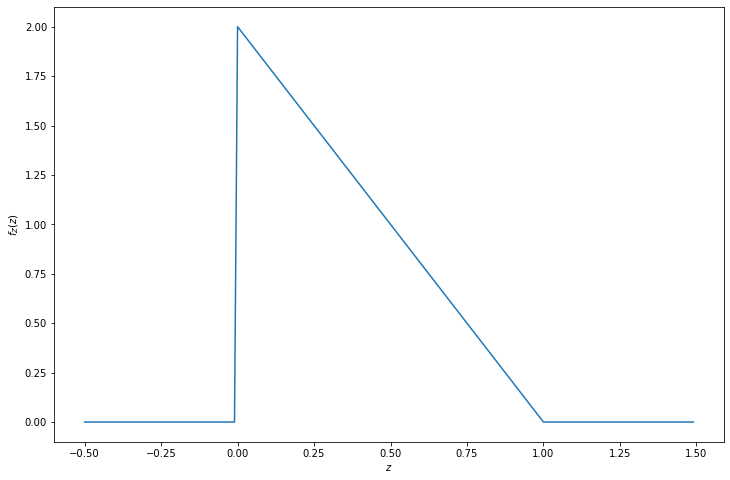
\includegraphics{Figure-03-06}
\end{figure}


\textbf{Exercise 3.14.8}. Let \(X\) have CDF \(F\). Find the CDF of
\(X^+ = \max \{0, X\}\).

\textbf{Solution}.
\[
F_{X^+}(x) = \PROB(X^+ \leq x) = \PROB(0 < x, X < x) = I(0 < x) F_X(x)
\]

\textbf{Exercise 3.14.9}. Let \(X \sim \text{Exp}(\beta)\). Find
\(F(x)\) and \(F^{-1}(q)\).

\textbf{Solution}. Start from the definition for the PDF of the
exponential distribution:
\[
f(x) = \frac{1}{\beta} e^{-x / \beta}, \quad x > 0
\]
We have:
\[
F(x) = \int_{-\infty}^x f(t) dt = \int_{-\infty}^x \frac{1}{\beta} e^{-t / \beta} dt = \frac{1}{\beta} \beta \left( 1 - e^{-x / \beta} \right) = 1 - e^{-x / \beta}
\]
and so
\[
q = 1 - e^{-F^{-1}(q) / \beta} \Longrightarrow F^{-1}(q) = -\beta \log (1 - q)
\]

\textbf{Exercise 3.14.10}. Let \(X\) and \(Y\) be independent. Show that
\(g(X)\) is independent of \(h(Y)\) where \(g\) and \(h\) are functions.

\textbf{Solution}. Let \(g^{-1}(A) = \{ x : g(x) \in A \}\) and
\(h^{-1}(B) = \{ y : h(y) \in B \}\). We have:
\begin{align*}
\PROB(g(X) \in A, h(Y) \in B) 
& = \PROB(X \in g^{-1}(A), Y \in h^{-1}(B) 
\\
& = \PROB(X \in g^{-1}(A)) \PROB(Y \in h^{-1}(B)) 
\\
& = \PROB(g(X) \in A) \PROB(h(Y) \in B)
\end{align*}

\textbf{Exercise 34.14.11}. Suppose we toss a coin once and let \(p\) be
the probability of heads. Let \(X\) denote the number of heads and \(Y\)
denote the number of tails.
\textbf{(a)} Prove that \(X\) and \(Y\) are dependent.
\textbf{(b)} Let \(N \sim \text{Poisson}(\lambda)\) and suppose that we
toss a coin \(N\) times. Let \(X\) and \(Y\) be the number of heads and
tails. Show that \(X\) and \(Y\) are independent.

\textbf{Solution}.
\textbf{(a)} The joint probability mass function is:
\[
\begin{array}{c|cc}
f_{X, Y} & Y = 0 & Y = 1 \\
\hline
X = 0 & 0 & 1 - p\\
X = 1 & p & 0
\end{array}
\]
In particular, \(f_{X, Y}(1, 0) = p\) and \(f_X(1) f_Y(0) = p^{2}\), so
the events are dependent unless \(p \in \{0, 1\}\).
\textbf{(b)} The joint probability mass function is:
\begin{align*}
\PROB(X = x, Y = y) 
  = \PROB(N = x + y, X = x) 
& = \frac{\lambda^{x+y}e^{-\lambda}}{(x + y)!} \binom{x + y}{x} p^x (1-p)^y 
\\[
1ex]
& = e^{-\lambda} \left(\frac{\lambda^x}{x!} p^x \right) \left(\frac{\lambda^y}{y!} (1 - p)^y\right) 
  = g(x) h(y)
\end{align*}
where \(g(x) =  \frac{e^{-\lambda}\lambda^x}{x!} p^{x}\), 
\(h(y) = \frac{\lambda^y}{y!} (1 - p)^{y} \). 
The result then follows from Theorem 3.33.

\textbf{Exercise 3.14.12}. Prove Theorem 3.33.
Suppose that the range of \(X\) and \(Y\) is a (possibly infinite)
rectangle. If \(f(x, y) = g(x) h(y)\) for some functions \(g\) and \(h\)
(not necessarily probability density functions) then \(X\) and \(Y\) are
independent.

\textbf{Solution}.
Given that \(F\) is the joint probability density function of \(X\) and
\(Y\), then the marginal distributions for \(X\) and \(Y\) are
\[
f_X(x) = \int f(x, y) dy = \int g(x) h(y) dy = g(x) \int h(y) dy = H g(x) \quad \text{ for some constant } H
\]
and
\[
f_Y(y) = \int f(x, y) dx = \int g(x) h(y) dx = h(y) \int g(x) dx = G h(y) \quad \text{ for some constant } G
\]
Therefore,
\[
f_X(x) f_Y(y) = HG g(x) h(y) = HG f(x, y)
\]
Integrating over \(x\), and fixing \(y = y_{0}\) with non-zero probability
density,
\[
\int f_X(x) f_Y(y_{0}) dx = HG \int f(x, y_{0}) dx \Longrightarrow f_Y(y_{0}) = HG f_Y(y_{0}) \Longrightarrow HG = 1
\]
and so
\[
f_X(x) f_Y(y) = f(x, y)
\]
therefore \(X\) and \(Y\) are independent.

\textbf{Exercise 3.14.13}. Let \(X \sim N(0, 1)\) and let \(Y = e^X\).
\textbf{(a)} Find the PDF for \(Y\). Plot it.
\textbf{(b) (Computer Experiment)} Generate a vector
\(x = (x_{1}, \dots, x_{10,000})\) consisting of 10,000 random standard
Normals. Let \(y = (y_{1}, \dots, y_{10,000})\) where \(y_{i} = e^{x_{i}}\).
Draw a histogram of \(y\) and compare it to the PDF you found in part
(a).

\textbf{Solution}.
\textbf{(a)}
Assuming \(y > 0\),
\[
F_Y(y) = \PROB(Y \leq y) = \PROB(X \leq \log y) = \Phi(\log y)
\]
and so
\[
f_Y(y) = \frac{d}{dy} \Phi(\log y) = \frac{d \Phi(\log y)}{d \log y} \frac{d \log y}{dy} = \frac{\phi(\log(y))}{y}
\]
And, of course, \(Y\) can never take a negative value, so
\[
f_Y(y) =
\begin{cases}
\frac{\phi(\log(y))}{y} &\text{if } y > 0 
\\[
1ex]
0 &\text{otherwise}
\end{cases}
\]

\begin{python}
import numpy as np
from scipy.stats import norm
import matplotlib.pyplot as plt
yy = np.arange(0.01, 5, step=0.01)
def f_Y(y):
    return norm.pdf(np.log(y)) / y
plt.figure(figsize=(12, 8))
plt.plot(yy, f_Y(yy))
plt.xlabel(r'$y$')
plt.ylabel(r'$f_Y(y)$')
plt.show()
\end{python}

\begin{figure}[H]
\centering
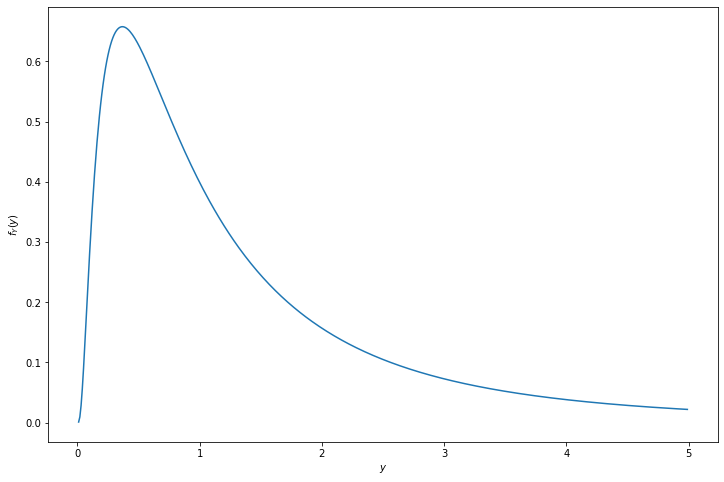
\includegraphics{Figure-03-07}
\end{figure}

\textbf{(b)}

\begin{python}
np.random.seed(0)
N = 10000
X = norm.rvs(size=N)
Y = np.exp(X)
plt.figure(figsize=(12, 8))
plt.hist(Y, bins=200, density=True, label='histogram', histtype='step')
plt.plot(yy, f_Y(yy), label='true density')
plt.legend(loc='upper right')
plt.xlim(0, 5)
plt.show()
\end{python}

\begin{figure}[H]
\centering
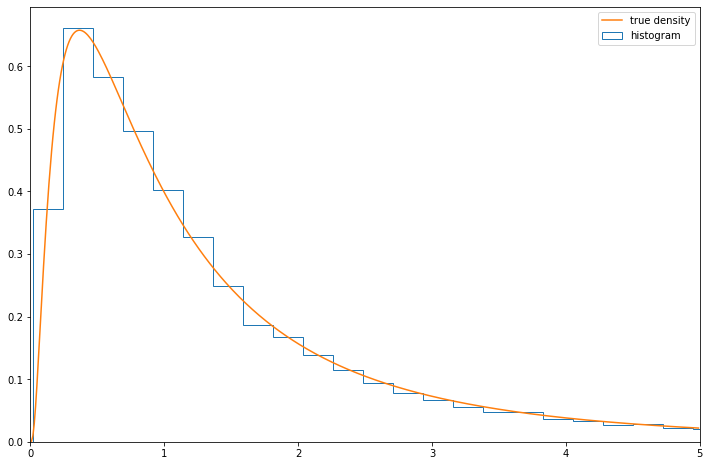
\includegraphics{Figure-03-08}
\end{figure}


\textbf{Exercise 3.14.14}. Let \((X, Y)\) be uniformly distributed on
the unit disc \(\{ (x, y) : x^{2} + y^{2} \leq 1 \}\). Let
\(R = \sqrt{X^{2} + Y^{2}}\). Find the CDF and the PDF of \(R\).

\textbf{Solution}.
Assuming \(r > 0\),
\[
F_R(r) = \PROB(R \leq r) = \PROB(X^{2} + Y^{2} \leq r^{2}) = \int \int_{x^{2} + y^{2} \leq r^{2}} f(x, y) dx dy
\]
is proportional to the area of a disc of radius \(r\). Since
\(F_R(1) = 1\), we have that the CDF is
\[
F_R(r) = \begin{cases}
0 &\text{if } r \leq 0 \\
r^{2} &\text{if } 0 < r \leq 1 \\
1 &\text{if } r > 1
\end{cases}
\]
and the PDF is \(f_R(r) = F'_R(r)\):
\[
f_R(r) = \begin{cases}
0 &\text{if } r \leq 0 \\
2 r &\text{if } 0 < r \leq 1 \\
0 &\text{if } r > 1
\end{cases}
\]

\textbf{Exercise 3.14.15 (A universal random number generator)}. Let
\(X\) have a continuous, strictly increasing CDF. Let \(Y = F(X)\). Find
the density of \(Y\). This is called the probability integral
transformation. Now let \(U \sim \text{Uniform}(0, 1)\) and let
\(X = F^{-1}(U)\). Show that \(X \sim F\). Now write a program that
takes \(\text{Uniform}(0, 1)\) random variables and generates random
variables from a \(\text{Exp}(\beta)\) distribution.

\textbf{Solution}.
For \(0 \leq y \leq 1\), the CDF of \(Y\) is
\[
F_Y(y) = \PROB(Y \leq y) = \PROB(F(X) \leq y) = \PROB(X \leq F^{-1}(y)) = F(F^{-1}(y)) = y
\]
and so \(Y \sim \text{Uniform}(0, 1)\).
For \(0 \leq q \leq 1\),
\[
F_X(q) = \PROB(X \leq q) = \PROB(F(X) \leq F(q)) = \PROB(U \leq F(q)) = F(q)
\]
and so \(X \sim F\).
To create a generator for \(\text{Exp}(\beta)\), let \(F\) be the CDF
for this distribution,
\[
F(x) = 1 - e^{-x/\beta} \quad F^{-1}(q) = - \beta \log (1 - q)
\]

\begin{python}
import numpy as np
def inv_F(beta):
    def inv_f_impl(q):
        return -beta * np.log(1 - q)
    return inv_f_impl
\end{python}

\begin{python}
np.random.seed(0)
N = 100000
U = np.random.uniform(low=0, high=1, size=N)
X = {}
for beta in [0.1, 1.0, 10.0]:
    X[beta] = inv_F(beta)(U)
\end{python}

\begin{python}
import matplotlib.pyplot as plt
from scipy.stats import expon
plt.figure(figsize=(12, 8))
for i, beta in enumerate([0.1, 1.0, 10]):
    ax = plt.subplot(3, 1, (i + 1))
    ax.hist(X[beta], density=True, bins=100, histtype='step', label='simulation histogram')
    xx = np.arange(beta * 0.01, 5 * beta, step=beta * 0.01)
    ax.plot(xx, expon.pdf(xx, scale=beta), label='true PDF')
    ax.set_xlim(-beta * 0.1, 5 * beta)
    ax.legend(loc='upper right')
    ax.set_title('beta = ' + str(beta))
    
plt.tight_layout()
plt.show()
\end{python}

\begin{figure}[H]
\centering
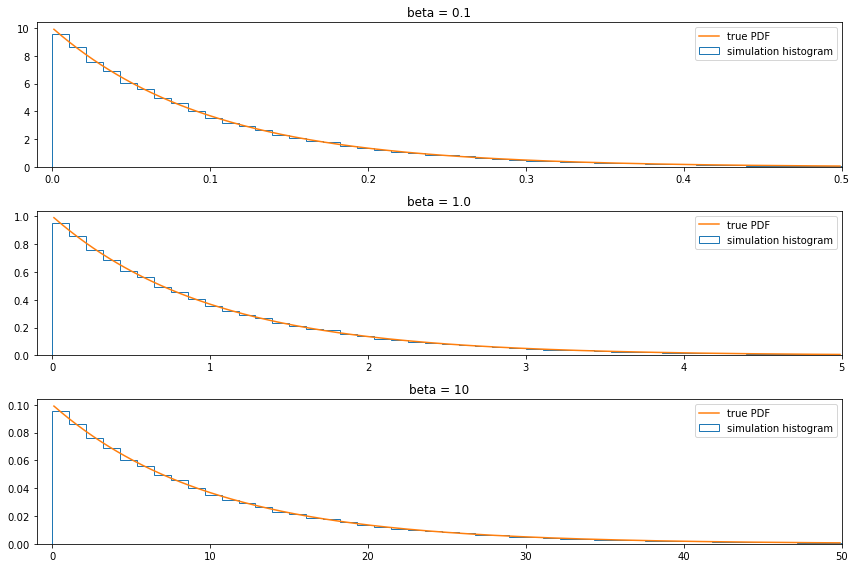
\includegraphics{Figure-03-09}
\end{figure}


\textbf{Exercise 3.14.16}. Let \(X \sim \text{Poisson}(\lambda)\) and
\(Y \sim \text{Poisson}(\mu)\) and assume that \(X\) and \(Y\) are
independent. Show that the distribution of \(X\) given that
\(X + Y = n\) is \(\text{Binomial}(n, \pi)\) where
\(\pi = \lambda / (\lambda + \mu)\).
Hint 1: You may use the following fact: If
\(X \sim \text{Poisson}(\lambda)\) and \(Y \sim \text{Poisson}(\mu)\),
and \(X\) and \(Y\) are independent, then
\(X + Y \sim \text{Poisson}(\mu + \lambda)\).
Hint 2: Note that \(\{X = x, X + Y = n\} = \{X = x, Y = n - x \}\)

\textbf{Solution}.
We have:
\begin{align*}
\PROB(X = x | X + Y = n) &= \frac{\PROB(X = x, X + Y = n)}{\PROB(X + Y = n)} \\
&= \frac{\PROB(X = x, Y = n - x)}{\PROB(X + Y = n)} \\
&= \frac{\PROB(X = x) \PROB(Y = n - x)}{\PROB(X + Y = n)} \\
&= \frac{\frac{\lambda^x e^{-\lambda}}{x!} \frac{\mu^{n - x} e^{-\mu}}{(n - x)!} }{\frac{(\lambda + \mu)^{n} e^{-(\lambda + \mu)}}{n!}} \\
&= \frac{n!}{x! (n - x)!} \frac{\lambda^x \mu^{n - x}}{(\lambda + \mu)^{n}} \\
&= \binom{n}{x} \left( \frac{\lambda}{\lambda + \mu} \right)^x \left( \frac{\mu}{\lambda + \mu}\right)^{n - x} \\
&= \binom{n}{x} \pi^x (1 - \pi)^{n - x}
\end{align*}
and so the result follows.

\textbf{Exercise 3.14.17}. Let
\[
f_{X, Y}(x, y) = 
\begin{cases}
c(x + y^{2}) &\text{if } 0 \leq x \leq 1 \text{ and }  0 \leq y \leq 1 
\\[
1ex]
0 & \text{otherwise}
\end{cases}
\]
Find \(\PROB\left( X < \frac{1}{2} | Y = \frac{1}{2} \right)\).

\textbf{Solution}.
The conditional density \(f_{X | Y}(x | y)\) is:
\[
f_{X|Y}(x | y) = \frac{f_{X, Y}(x, y)}{f_Y(y)} = \frac{f_{X, Y}(x, y)}{\int f_{X, Y}(t, y) dt}
= \frac{ c(x + y^{2}) }{\int_{0}^{1} c(t + y^{2}) dt} =  \frac{ x + y^{2} }{\int_{0}^{1} t + y^{2} dt} = \frac{x + y^{2}}{\frac{1}{2} + y^{2}}
\]
In particular, when \(y = 1/2\),
\[
f_{X|Y}(x | 1/2) = \frac{4x + 1}{3}
\]
and so
\[
\PROB\left( X < x \;\Bigg|\; Y = \frac{1}{2} \right) = \int_{0}^x \frac{4t + 1}{3} dt = \frac{2x^{2} + x}{3}
\]
so
\[
\PROB\left( X < \frac{1}{2} \;\Bigg|\; Y = \frac{1}{2} \right) = \frac{1}{3}
\]
\textbf{Exercie 3.14.18}. Let \(X \sim N(3, 16)\). Solve the following
using the Normal table and using a computer package.
\textbf{(a)} Find \(\PROB(X < 7)\).
\textbf{(b)} Find \(\PROB(X > -2)\).
\textbf{(c)} Find \(x\) such that \(\PROB(X > x) = .05\).
\textbf{(d)} Find \(\PROB(0 \leq X < 4)\).
\textbf{(e)} Find \(x\) such that \(\PROB(|X| > |x|) = .05\).

\textbf{Solution}.
Rather than using tables, we will express these in terms of a standard
Normal, and use ``computer packages'' to compute the expression based
both on the original Normal and the standard Normal.
\textbf{(a)}
\(\PROB(X < 7) = \PROB\left(\frac{X - 3}{4} < \frac{7 - 3}{4} \right) = \PROB\left(Z < 1 \right) = \Phi\left( 1 \right)\)

\begin{python}
import numpy as np
from scipy.stats import norm
print('%.4f' % norm.cdf(1))
print('%.4f' % norm.cdf(7, loc=3, scale=4))
\end{python}
\begin{console}
0.8413
0.8413
\end{console}
\textbf{(b)} $\PROB(X > -2) =
\PROB\left(\frac{X - 3}{4} > \frac{-2 - 3}{4} \right)
= \PROB\left(Z < -\frac{5}{4} \right) = 1 - \Phi\left(
-\frac{5}{4} \right) $

\begin{python}
import numpy as np
from scipy.stats import norm
print('%.4f' % (1 - norm.cdf(-5/4)))
print('%.4f' % (1 - norm.cdf(-2, loc=3, scale=4)))
\end{python}
\begin{console}
0.8944
0.8944
\end{console}
\textbf{(c)} \(\PROB(X > x) = .05
\Longleftrightarrow 1 - F_X(x) = .05
\Longleftrightarrow F_X(x) = .95
\Longleftrightarrow x = F_X^{-1}(.95)\)
or: \(\PROB(X > x) = .05
\Longleftrightarrow \PROB\left(\frac{X - 3}{4} > \frac{x - 3}{4}\right) = .05
\Longleftrightarrow 1 - \Phi\left(\frac{x - 3}{4}\right) = .05
\Longleftrightarrow \frac{x - 3}{4} = \Phi^{-1}(.95)
\Longleftrightarrow x = 4 \Phi^{-1}(.95) + 3\)

\begin{python}
import numpy as np
from scipy.stats import norm
print('%.4f' % norm.ppf(.95, loc=3, scale=4))
print('%.4f' % (4 * norm.ppf(.95) + 3))
\end{python}
\begin{console}
9.5794
9.5794
\end{console}
\textbf{(d)} \(\PROB(0 \leq X < 4) = F_X(4) - F_X(0)\)
or
\(\PROB(0 \leq X < 4) = \PROB\left(\frac{0 - 3}{4} < Z < \frac{4 - 3}{4} \right) = \Phi\left( \frac{1}{4} \right) - \Phi\left( \frac{-3}{4} \right)\)

\begin{python}
import numpy as np
from scipy.stats import norm
print('%.4f' % (norm.cdf(4, loc=3, scale=4) - norm.cdf(0, loc=3, scale=4)))
print('%.4f' % (norm.cdf(1/4) - norm.cdf(-3/4)))
\end{python}
\begin{console}
0.3721
0.3721
\end{console}
\textbf{(e)} \(\PROB(|X| > |x|) = .05\)
For a constant \(c \geq 0\), we have
\begin{align*}
\PROB(|X| > c) &= 1 - \PROB(|X| < c) = 1 - \PROB(-c < X < -c) \\
&= 1 - \PROB\left( -\frac{c - 3}{4} < Z < \frac{c - 3}{4} \right)\\
&= 1 - \Phi\left( \frac{c - 3}{4} \right) + \Phi\left( -\frac{c - 3}{4} \right) \\
&= 2 - 2 \Phi\left( \frac{c - 3}{4} \right) = 2 - 2 F_X(c)
\end{align*}
So we can solve the original equation:
\[
2 - 2 F_X(c) = .05 \Longleftrightarrow c = F_X^{-1}(0.975)
\]
or
\[
2 - 2 \Phi\left( \frac{c - 3}{4} \right) = .05 \Longleftrightarrow c = 4 \Phi^{-1}(0.975) + 3
\]

\begin{python}
import numpy as np
from scipy.stats import norm
print('%.4f' % (norm.ppf(0.975, loc=3, scale=4)))
print('%.4f' % (4 * norm.ppf(0.975) + 3))
\end{python}
\begin{console}
10.8399
10.8399
\end{console}

\textbf{Exercise 3.14.19}. Prove formula (3.11).
Given \(Y = r(X)\), when \(r\) is strictly monotone increasing or
strictly monotone decreasing then \(r\) has an inverse \(s = r^{-1}\)
and in this case one can show that
\[
f_Y(y) = f_X(s(y)) \;\Bigg| \frac{ds(y)}{dy} \Bigg|
\]

\textbf{Solution}.
Assume \(r\) is strictly monotone increasing. Then $ \frac{d s(y)}{dy}
> 0$, and the CDF of \(Y\) is
\[
F_Y(y) = \PROB(Y \leq y) = \PROB(r(X) \leq y) = \PROB(X \leq s(y)) = F_X(s(y))
\]
Derivating over \(y\),
\begin{align*}
\frac{d}{dy} F_y(y) &= \frac{d F_X(s(y))}{d s(y)} \frac{d s(y)}{dy} \\
f_Y(y) &= f_X(s(y)) \frac{d s(y)}{dy}
\end{align*}
For the case when \(r\) is strictly monotone decreasing, $
\frac{d s(y)}{dy} < 0$, and the CDF of \(Y\) is
\[
F_Y(y) = \PROB(Y \leq y) = \PROB(r(X) \leq y) = \PROB(X \geq s(y)) = 1 - F_X(s(y))
\]
Derivating over \(y\),
\begin{align*}
\frac{d}{dy} F_y(y) &= \frac{d -F_X(s(y))}{d s(y)} \frac{d s(y)}{dy} \\
f_Y(y) &= -f_X(s(y)) \frac{d s(y)}{dy}
\end{align*}
and the result follows.

\textbf{Exercise 3.14.20}. Let \(X, Y \sim \text{Uniform}(0, 1)\) be
independent. Find the PDF for \(X - Y\) and \(X / Y\).

\textbf{Solution}.
The joint density of \(X, Y\) is
\[
f(x, y) = 
\begin{cases}
1 &\text{if } 0 \leq x \leq 1, 0 \leq y \leq 1 
\\[
1ex]
0 &\text{otherwise}
\end{cases}
\]
Let \(A = X - Y\). The CDF of \(A\) is calculated over the area
\(A_a = \{ (x, y) : x - y \leq a \}\):
\[
F_A(a) = \PROB(X + Y \leq a) = \int_{A_a} f(x, y)\; dx dy
\]
\begin{itemize}
\item
  If \(0 \leq a \leq 1\), the area is consists of all points in the unit
  square, othe than the triangle at points
  \((a, 0), (1, 0), (1, 1 - a)\). Then,
  \[
F_A(a) = 1 - \frac{(1 - a)^{2}}{2}
\]
\item
  If \(-1 \leq a \leq 0\), the area consists of only the points in the
  triangle \((0, 1), (1 + a, 1), (0, -a)\). Then,
  \[
F_A(a) = \frac{(1 + a)^{2}}{2}
\]
\end{itemize}
Therefore, the PDF is \(f_A(a) = F'_A(a)\), or
\[
f_A(a) =
\begin{cases}
1 + a &\text{if } -1 < a \leq 0
\\[
1ex]
1 - a &\text{if } 0 < a \leq 1
\\[
1ex]
0 &\text{otherwise}
\end{cases} 
\]

\begin{python}
import numpy as np
import matplotlib.pyplot as plt
plt.figure(figsize=(8, 4))
ax = plt.subplot(1, 2, 1)
a = 1/3
x = [0, a, 1, 1, 0]
y = [0, 0, 1 - a, 1, 1]
ax.fill(x, y)
ax.set_xlim(-0.5, 1.5)
ax.set_ylim(-0.5, 1.5)
ax.set_title('a = 1/3')
ax = plt.subplot(1, 2, 2)
a = -1/3
x = [0, 1+a, 0]
y = [1, 1, -a]
ax.fill(x, y)
ax.set_xlim(-0.5, 1.5)
ax.set_ylim(-0.5, 1.5)
ax.set_title('a = -1/3')
plt.tight_layout()
plt.show()
\end{python}

\begin{figure}[H]
\centering
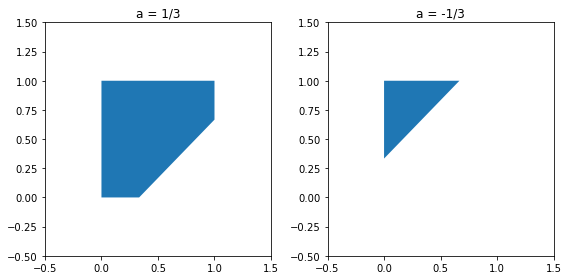
\includegraphics{Figure-03-10}
\end{figure}

Let \(B = X/Y\). The CDF of \(B\) is calculated over the area
\(B_b = \left\{ (x, y) : \frac{x}{y} \leq b \right\}\).
\[
F_B(a) = \PROB\left(\frac{X}{Y} \leq b\right) = \int_{B_b} f(x, y)\; dx dy
\]
\begin{itemize}
\item
  If \(0 < b \leq 1\), the relevant area is a triangle with points
  \((0, 0), (1, 0), (1, b)\). Then,
  \[
F_B(b) = \frac{b}{2}
\]
\item
  If \(b > 1\), the relevant area is the unit square minus the triangle
  with points \((0, 0), (0, 1), (1/b, 1)\). Then,
  \[
F_B(b) = 1 - \frac{1}{2b}
\]
\end{itemize}
Therefore, the PDF is \(f_B(b) = F'_B(b)\), or
\[
f_A(a) =
\begin{cases}
\frac{1}{2} &\text{if } 0 < b \leq 1
\\[
1ex]
\frac{1}{2b^{2}} &\text{if } b > 1
\\[
1ex]
0 &\text{otherwise}
\end{cases}
\]

\begin{python}
import numpy as np
import matplotlib.pyplot as plt
plt.figure(figsize=(8, 4))
ax = plt.subplot(1, 2, 1)
b = 1/3
x = [0, b, 0]
y = [0, 1, 1]
ax.fill(x, y)
ax.set_xlim(-0.5, 1.5)
ax.set_ylim(-0.5, 1.5)
ax.set_title('b = 1/3')
ax = plt.subplot(1, 2, 2)
b = 3
x = [0, 1, 1, 0]
y = [0, 1/b, 1, 1]
ax.fill(x, y)
ax.set_xlim(-0.5, 1.5)
ax.set_ylim(-0.5, 1.5)
ax.set_title('b = 3')
plt.tight_layout()
plt.show()
\end{python}

\begin{figure}[H]
\centering
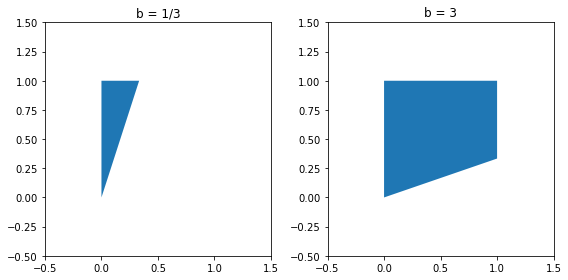
\includegraphics{Figure-03-11}
\end{figure}


\textbf{Exercise 3.14.21}. Let
\(X_{1}, \dots, X_{n} \sim \text{Exp}(\beta)\) be IID. Let
\(Y = \max \{ X_{1}, \dots, X_{n} \}\). Find the PDF of \(Y\). Hint:
\(Y \leq y\) if and only if \(X_{i} \leq y\) for \(i = 1, \dots, n\).

\textbf{Solution}. We have:
\[
\PROB(Y \leq y) = \PROB(\forall i, X_{i} \leq y) = \prod_{i} \PROB(X_{i} \leq y) = \prod_{i} \left(1 - e^{-y/\beta}\right) = (1 - e^{-y/\beta})^{n}
\]
and so the PDF is \(f_Y(y) = F'_Y(y)\):
\[
f_Y(y) = \frac{d (1 - e^{-y/\beta})^{n}}{dy} = \frac{n}{\beta} e^{-y/\beta} (1 - e^{-y/\beta})^{n-1}
\]

\textbf{Exercise 3.14.22}. Let \(X\) and \(Y\) be random variables.
Suppose that \(\EXP(Y | X) = X\). Show that
\(\COV(X, Y) = \VAR(X)\).

\textbf{Solution}.
The covariance is:
\[
\COV(X, Y) = \EXP(XY) - \EXP(X) \EXP(Y)
\]
and the variance is
\[
\VAR(X) = \EXP(X^{2}) - \EXP(X)^{2}
\]
We aim to prove that both of those expressions have the same value when
\(\EXP(Y | X) = X\).
Taking the expectaion on \(\EXP(Y | X)\) we get:
\[
\EXP(\EXP(Y | X)) = \int \EXP(Y = y | X) f_Y(y) \; dy = \int y f_Y(y) = \EXP(Y)
\]
so taking the expectation on both sides of \(\EXP(Y | X) = X\)
gives us \(\EXP(Y) = \EXP(X)\).
Now, we have
\begin{align*}
\EXP(XY) &= \int \EXP(XY | X = x) f_X(x) dx \\
&= \int \EXP(xY | X = x) f_X(x) dx \\
&= \int x \EXP(Y | X = x) f_X(x) dx \\
&= \int x^{2} f_X(x) dx \\
&= \EXP(X^{2})
\end{align*}
Using \(\EXP(X^{2}) = \EXP(XY)\) and
\(\EXP(Y) = \EXP(X)\), we get the desired result.

\textbf{Exercise 3.14.23}. Let \(X \sim \text{Uniform}(0, 1)\). Let
\(0 < a < b < 1\). Let
\[
Y =
\begin{cases}
1 &\text{if } 0 < x < b
\\[
1ex]
0 &\text{otherwise}
\end{cases}
\]
and let
\[
Z =
\begin{cases}
1 &\text{if } a < x < 1 
\\[
1ex]
0 &\text{otherwise}
\end{cases}
\]
\textbf{(a)} Are \(Y\) and \(Z\) independent? Why / Why not?
\textbf{(b)} Find \(\EXP(Y | Z)\). Hint: what values \(z\) can
\(Z\) take? Now find \(\EXP(Y | Z = z)\).

\textbf{Solution}.
\textbf{(a)} The joint probability mass function for \(Y\) and \(Z\) is:
\[
\begin{array}{c|cc}
 & Z = 0 & Z = 1 \\
\hline
Y = 0 & 0 & 1 - b \\
Y = 1 & a & b - a
\end{array}
\]
These are not independent; in particular,
\[
\PROB(Y = 1, Z = 1) = b - a \neq \PROB(Y = 1) \PROB(Z = 1) = b(1 - a)
\]
since the equality would only hold if \(b = 0\) or \(a = 0\), and the
inequality precludes both of these.
\textbf{(b)} We have:
\[
\EXP(Y | Z = 0) = \frac{\sum_y y f(y, 0)}{f_Z(0)} = \frac{f(1, 0)}{a} = 1
\]
and
\[
\EXP(Y | Z = 1) = \frac{\sum_y y f(y, 1)}{f_Z(1)} = \frac{f(1, 1)}{1 - a} = \frac{b - a}{1 - a}
\]
